\documentclass[12pt, twoside]{article}
\usepackage{jmlda}
\newcommand{\hdir}{.}
\usepackage[utf8]{inputenc}
\usepackage[english,russian]{babel}
\usepackage{graphicx}
\newcommand{\real}{\mathbb{R}}
\newcommand{\nat}{\mathbb{N}}
\newcommand{\integ}{\mathbb{Z}}
\usepackage{bm}
\usepackage{multicol}
\usepackage{comment}
\begin{document}

\title
    [Анализ свойств ансамбля локально аппроксимирующих моделей] % краткое название; не нужно, если полное название влезает в~колонтитул
    {Анализ свойств ансамбля локально аппроксимирующих моделей}
\author
    [Р.\,И.~Исламов, А.\,В.~Грабовой, В.\,В.~Стрижов] % список авторов (не более трех) для колонтитула; не нужен, если основной список влезает в колонтитул
    {Р.\,И.~Исламов, А.\,В.~Грабовой, В.\,В.~Стрижов} % основной список авторов, выводимый в оглавление
    [Р.\,И.~Исламов$^1$, А.\,В.~Грабовой$^1$, В.\,В.~Стрижов$^{1}$] % список авторов, выводимый в заголовок; не нужен, если он не отличается от основного
\email
    {islamov.ri@phystech.edu; grabovoy.av@phystech.edu;  strijov@ccas.ru}
%\thanks
%    {Работа выполнена при
%     %частичной
%     финансовой поддержке РФФИ, проекты \No\ \No 00-00-00000 и 00-00-00001.}
\organization
    {$^1$Московский физико-технический институт}
\abstract
    {Данная работа посвящена построению универсальной модели в виде ансамбля локальных моделей. Для решения задачи регрессии  предлагается использовать многоуровневый подход. Множество объектов выборки разбивается на несколько подмножеств, каждому подмножеству ставится в соответствие одна локальная модель, оптимально аппроксимирующая данное подмножество. Для аппроксимации генеральной выборки строится универсальный аппроксиматор, который представлен в виде ансамбля локальных моделей. В качестве коэффициентов шлюзовой функции используется выпуклая комбинация локальных моделей, значение которой зависит от объекта, для которого производится предсказание. Ансамблевый подход позволяет описывать те выборки, которые затруднительно описать одной моделью. Для анализа свойств проводится вычислительный эксперимент. В качестве данных используются синтетические и реальные выборки.   
	
\bigskip
\noindent
\textbf{Ключевые слова}: \emph {локальная модель; линейные модели; ансамбль моделей.}
}

\maketitle
\linenumbers

\section{Введение}

В прикладных задачах данные порождены несколькими источниками. В таких случаях качество предсказания можно повышать увеличивая число моделей. Если моделей на самом деле меньше, чем предполагается, то веса лишних моделей будут малы и их вклад
будет несущественен. Преимуществом ансамбля является его способность описывать те выборки, которые затруднительно описывать одной моделью.

В данной работе исследуется проблема построения ансамбля локальных моделей. \textit{Локальная модель} --- модель, которая аппроксимирует объекты, находящиеся в одной связной области в пространстве объектов. В качестве решающей функции используется выпуклая комбинация локальных моделей, при этом веса локальных моделей не постоянны, а зависят от положения объекта в пространстве объектов. 

Ансамблевый подход предполагает, что вклад каждой локальной модели в целевую переменную зависит от рассматриваемого объекта. Ансамбль локальных моделей использует шлюзовую функцию, которая определяет значимость предсказания каждой локальной модели, входящей в ансамбль.

В данной работе каждая локальная модель является линейной. В качестве функции ошибки используется логарифм правдоподобия модели. Оптимальные параметры ансамбля и локальных моделей находятся при решении двухуровневой задачи оптимизации. 



Алгоритмы тестировались на синтетических и реальных данных.  Эксперименты показали преимущество использования многоуровневой модели и смеси моделей по сравнению с использованием одной модели.






С момента своего появления ансамблевый подход стал предметом многих исследований. Ансамбль моделей использовался в работах\cite{Yumlu2003}, \cite{Cheung1995}, \cite{Weigend2000}. В работе \cite{Yuksel2012} представлен обзор методов и моделей в задачах ансамбля моделей. В данной работе представлены виды шлюзовых функций. Приведен анализ разных моделей, которые могут выступать в качестве локальной модели. 

Ансамблевый подход имеет множество приложений в прикладных задачах. В работе \cite{article} предложен метод распознавания рукописных цифр. Метод распознания текстов при помощи ансамбля локальных моделей исследуется в работах \cite{Estabrooks2001}, а для распознавания речи --- в \cite{Mossavat2010}, \cite{Peng1996}. В работе \cite{Sminchisescu2007} исследуется смесь экспертов для задачи распознавания трехмерных движений человека.


Были предложены различные типы локальных моделей, такие как SVM \cite{Collobert2002}, Гауссовский процесс \cite{Tresp01mixturesof}  и нейронные сети \cite{Shazeer2017}. Другие работы была сосредоточены на различных конфигурациях, таких как иерархическая структура \cite{NIPS1991_514}, бесконечное число экспертов \cite{Rasmussen} и последовательное добавление экспертов \cite{Aljundi2016}. \cite{garmash-monz-2016-ensemble} предлагает модель ансамбля локальных моделей для машинного перевода. Стробирующая сеть обучается на предварительно обученной модели NMT ансамбля. 



\section{Постановка задачи построения ансамбля локальных моделей}

Пусть задано множество объектов $\Omega$, признаки которых описываются матрицей
\[\mathbf{X} \in \real^{N\times n}, \eqno(2.1)\]
где $N$ --- число объектов во множестве, а $n$ --- размерность признакового пространства. Каждому объекту $\omega_i$ из $\Omega$ соответствует признаковое описание $\mathbf{x}_i \in \real^n$, которое является $i$-ой строкой матрицы $\mathbf{X}$, и значение целевой переменной $y_i \in \real$.  Введем выборку данных $\mathfrak{D}$:
\[\mathfrak{D} = \{(\mathbf{x}_i, y_i)~|~ i \in \overline{1, N}\}. \eqno(2.2)\]

Будем считать, что множество индексов $I = \{1, 2, \dotsc, N\}$ разбивается на $K$ непересекающихся подмножеств $I_k$:

\[I = \bigcup\limits_{k=1}^K I_k. \eqno(2.3)\]
Разбиение индексного множества $I$ индуцирует разбиение множества объектов $\Omega$ на подмножества $\Omega_k$
\[\Omega = \bigcup\limits_{k=1}^K \Omega_k, \qquad \Omega_k = \{\omega_i \in \Omega~|~i \in I_k\}\eqno(2.4)\]
и выборку $\mathfrak{D}$ на подвыборки $\mathfrak{D}_k$
\[\mathfrak{D} = \bigcup\limits_{k=1}^K \mathfrak{D}_k, \qquad \mathfrak{D}_k = \{(\mathbf{x}_i, y_i) \in \mathfrak{D}~|~i \in I_k\}\eqno(2.5)\]
Для каждого подмножества объектов $\Omega_k$ используется своя локальная модель.\\
\begin{Definition}
\label{def:1}
Модель $\mathbf{g}_k$ называется локальной, если она аппроксимирует аппроксимирует подвыборку $\mathfrak{D}_k = \{(\mathbf{x}_i, y_i) \in \mathfrak{D}~|~i \in I_k\}$.
\end{Definition}
В данной работе локальный модели объединены в ансамбль локальных моделей.\\
\begin{Definition}
\label{def:2}
Ансамбль локальных моделей --- мультимодель, определяющая правдоподобие веса $\pi_k$ каждой локальной модели $\textbf{g}_k$ на признаковом описании объекта $\textbf{x}$.
\[\mathbf{f} = \sum\limits_{k=1}^K\pi_k\mathbf{g}_k(\mathbf{x},\mathbf{w}_k),\qquad \pi_k\left(\mathbf{x}, \mathbf{V}\right): \real^{n\times |\mathbf{V}|} \rightarrow [0,1], \qquad \sum\limits_{k=1}^K\pi_k\left(\mathbf{x}, \mathbf{V}\right) = 1, \eqno(2.6)\]
где $\mathbf{f}$ --- мультимодель, $\mathbf{g}_k$ --- локальная модель, $\pi_k$ --- шлюзовая функция, $\mathbf{V}$--- параметры шлюзовой функции. 
\end{Definition}



В работе в качестве локальной модели $\mathbf{g}_k$ и шлюзовой функции $\bm{\pi}$ рассматриваются следующие функции:

\[\mathbf{g}_k(\mathbf{x}, \mathbf{w}_k) = \mathbf{w}_k^{\mathsf{T}}\mathbf{x}, \qquad \bm{\pi}\left(\mathbf{x}, \mathbf{V}\right) = \text{softmax}\bigg(\mathbf{V}_1^{\mathsf{T}}\sigma\left(\mathbf{V}_2^{\mathsf{T}}\mathbf{x}\right)\bigg), \eqno(2.7)\]
где $\mathbf{V} = \{\mathbf{V}_1, \mathbf{V}_2\}$ --- параметры шлюзовой функции, $\sigma(x)$ --- сигмоидная функция. Введем понятие расстояние между двумя объектами.\\
\begin{Definition}
\label{def:3}
Расстоянием между двумя объектами $\omega_1$ и $\omega_2$ из $\Omega$ называется число, равное расстоянию между векторами $\mathbf{x}_1, \mathbf{x}_2$ признаковых описаний этих объектов:

\[\rho(\omega_1, \omega_2) = ||\mathbf{x}_1 - \mathbf{x}_2||_2. \eqno(2.8) \] 
\end{Definition} 
Будем считать, что каждый объект имеет признаковое описание $\mathbf{x}$, взятый из некоторого вероятностного распределения. Пусть этому распределению соответствует вероятностная мера $\mathsf{F}(x)$ в пространстве признаков. Тогда пространство локальных моделей является гильбертовым пространством, в котором введено скалярное произведение.\\
\begin{Definition}
\label{def:2}
Скалярным произведением между двумя локальными моделями $\mathbf{g}_i$ и $\mathbf{g}_j$ называется число, вычисляемое по формуле
\[ \left<\mathbf{g}_i, \mathbf{g}_j\right> = \mathsf{E}\bigg(\mathbf{g}_i(\mathbf{x}\cdot \mathbf{w}_i)\cdot\mathbf{g}_j(\mathbf{x}, \mathbf{w}_j) \bigg), \eqno(2.9)\]
где $\mathsf{E}\left(\xi\cdot \eta\right) = \int\limits_{\real^n}\xi(\mathbf{x})\eta(\mathbf{x})\mathsf{dF}(\mathbf{x})$ --- математическое ожидание произведения случайных величин.
\end{Definition}


Для нахождения оптимальных параметров мультимодели используется функция ошибки следующего вида:
\[\mathcal{L}\left(\textbf{V}, \textbf{W}\right) = \sum\limits_{(\textbf{x}, y) \in \mathcal{D}} \sum\limits_{k=1}^K\pi_k\left(\textbf{x}, \textbf{V}\right)\left(y - \textbf{w}_k^{\mathsf{T}}\textbf{x}^k\right)^2 + R\left(\mathbf{V}, \mathbf{W}\right), \eqno(2.10)\] 
где $\mathbf{W} = [\mathbf{w}_1, \mathbf{w}_2, \dotsc, \mathbf{w}_k]$ --- параметры локальных моделей, $R\left(\mathbf{V}, \mathbf{W}\right)$ --- регуляризация параметров. Оптимальные параметры определяются из выражения

\[\hat{\mathbf{V}}, \hat{\mathbf{W}} = \argmin\limits_{\mathbf{V}, \mathbf{W}}{\mathcal{L}\left(\textbf{V}, \textbf{W}\right)}. \eqno(2.11)\]

\section{Вычислительный эксперимент}

\subsection{Постановка проблемы}

Данный эксперимент ставится для того, чтобы показать, что одна линейная модель плохо аппроксимирует выборку, объекты которой порождены несколькими источниками. 

В качестве данных используются синтетическая выборка. Создается две подвыборки объектов, имеющих по одному признаку $x^k$, описываемых линейной моделью с нормальным шумом:
\[\mathbf{y}_k = \alpha_{k}\mathbf{x}^k+ \bm\varepsilon, \qquad k \in \{1,2\},  \qquad x_k,y_k \in \real,\qquad \varepsilon \in \mathcal{N}(0, 1). \eqno(3.1)\] 
Эти две подвыборки сливаются в одну общую выборку, описываемую вектором целевой переменной $\mathbf{y}$ и матрицей признаков $\mathbf{X}$:
\[\mathbf{y} = \begin{pmatrix}
\mathbf{y}_1\\
\mathbf{y}_2
\end{pmatrix}, \qquad\mathbf{X} = \begin{pmatrix}
\mathbf{x}^1 & \mathbf{0}\\
\mathbf{0} & \mathbf{x}^2
\end{pmatrix}.\eqno(3.2)\]

На общей выборке обучается линейная модель. Линейная модель хорошо аппроксимирует данную выборку (см. рис. $1\text{a}$). 

Во втором эксперименте две подвыборки сливаются в одну общую выборку, описываемая целевой переменной $\mathbf{y}$ и матрицей признаков $\hat{\mathbf{X}}$:
\[\mathbf{y} = \begin{pmatrix}
\mathbf{y}_1\\
\mathbf{y}_2
\end{pmatrix}, \qquad \mathbf{\hat{X}} = \begin{pmatrix}
\mathbf{x}^1 & \bm\varepsilon_1\\
\bm\varepsilon_2 & \mathbf{x}^2
\end{pmatrix},\eqno(3.2)\]
где $\bm\varepsilon_1, \bm\varepsilon_2 \in \mathcal{N}(0,1)$. На построенной модели также обучается линейная модель. В этом случае линейная модель плохо аппроксимирует данную выборку (см. рис. $1\text{б}$). 




\begin{figure}[h]
\begin{center}
\begin{minipage}[h]{0.49\linewidth}
\begin{center}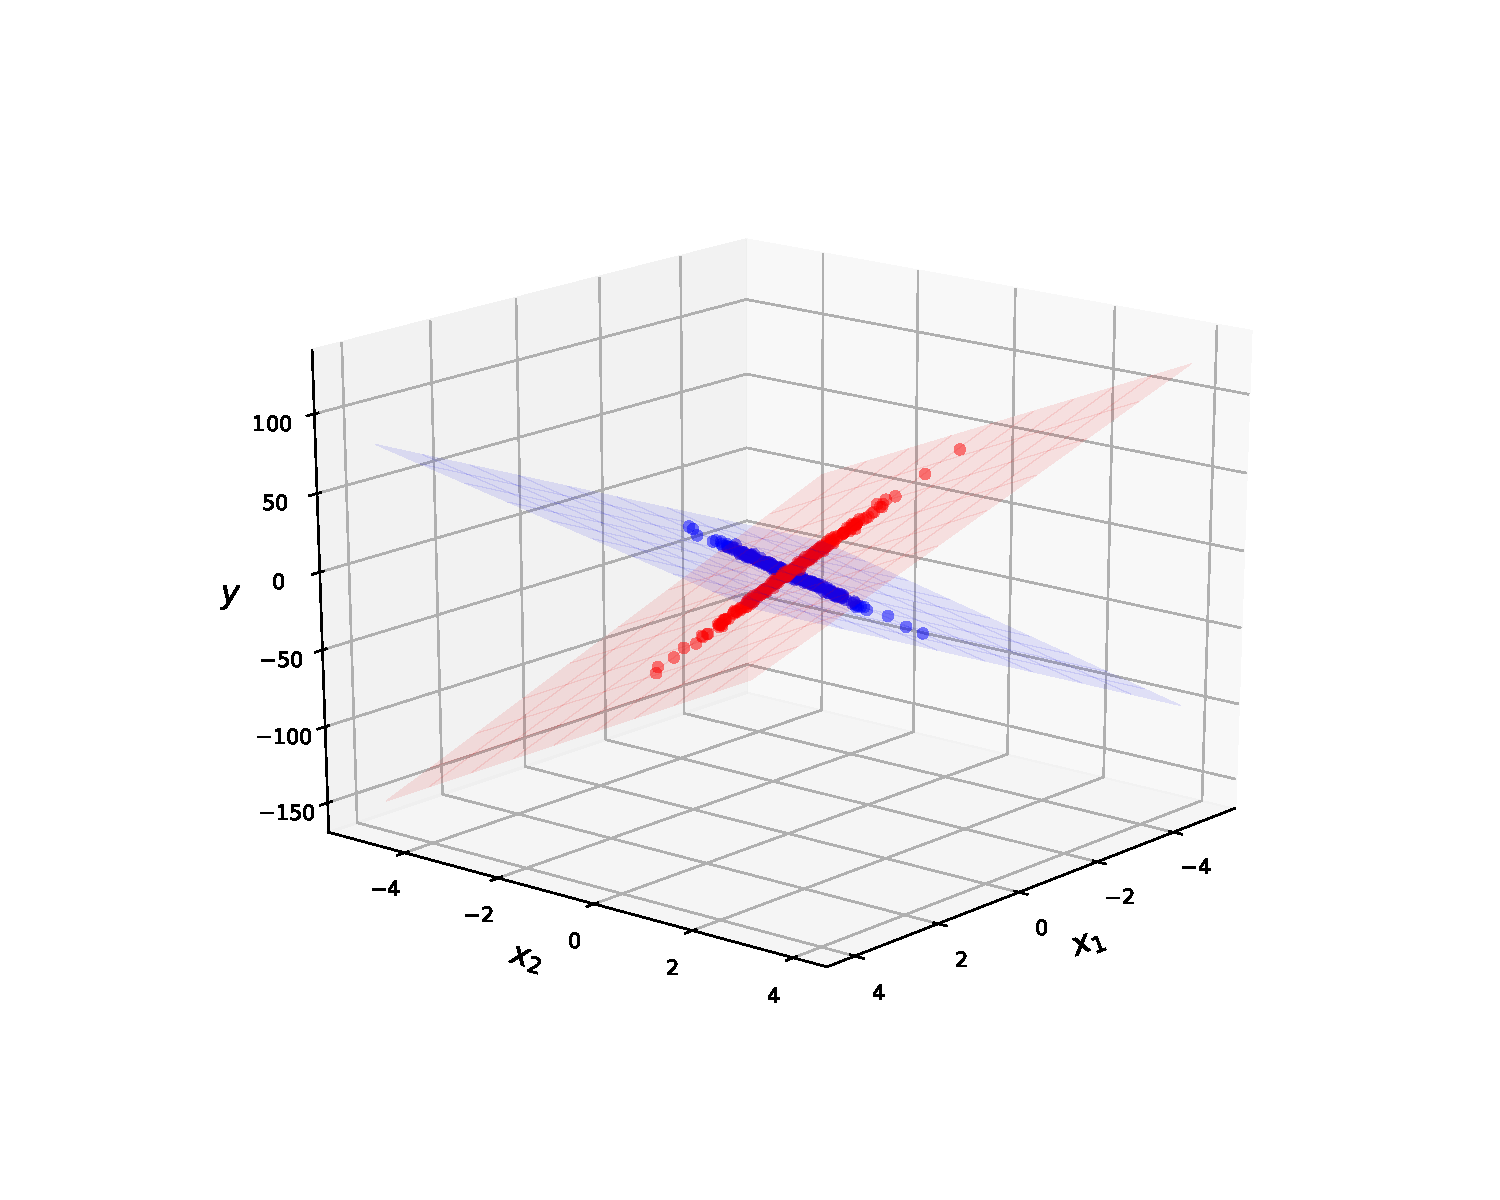
\includegraphics[width=1.2\linewidth]{experiment1-zeros.pdf}  а) \end{center}
\end{minipage}
\hfill
\begin{minipage}[h]{0.49\linewidth}
\begin{center}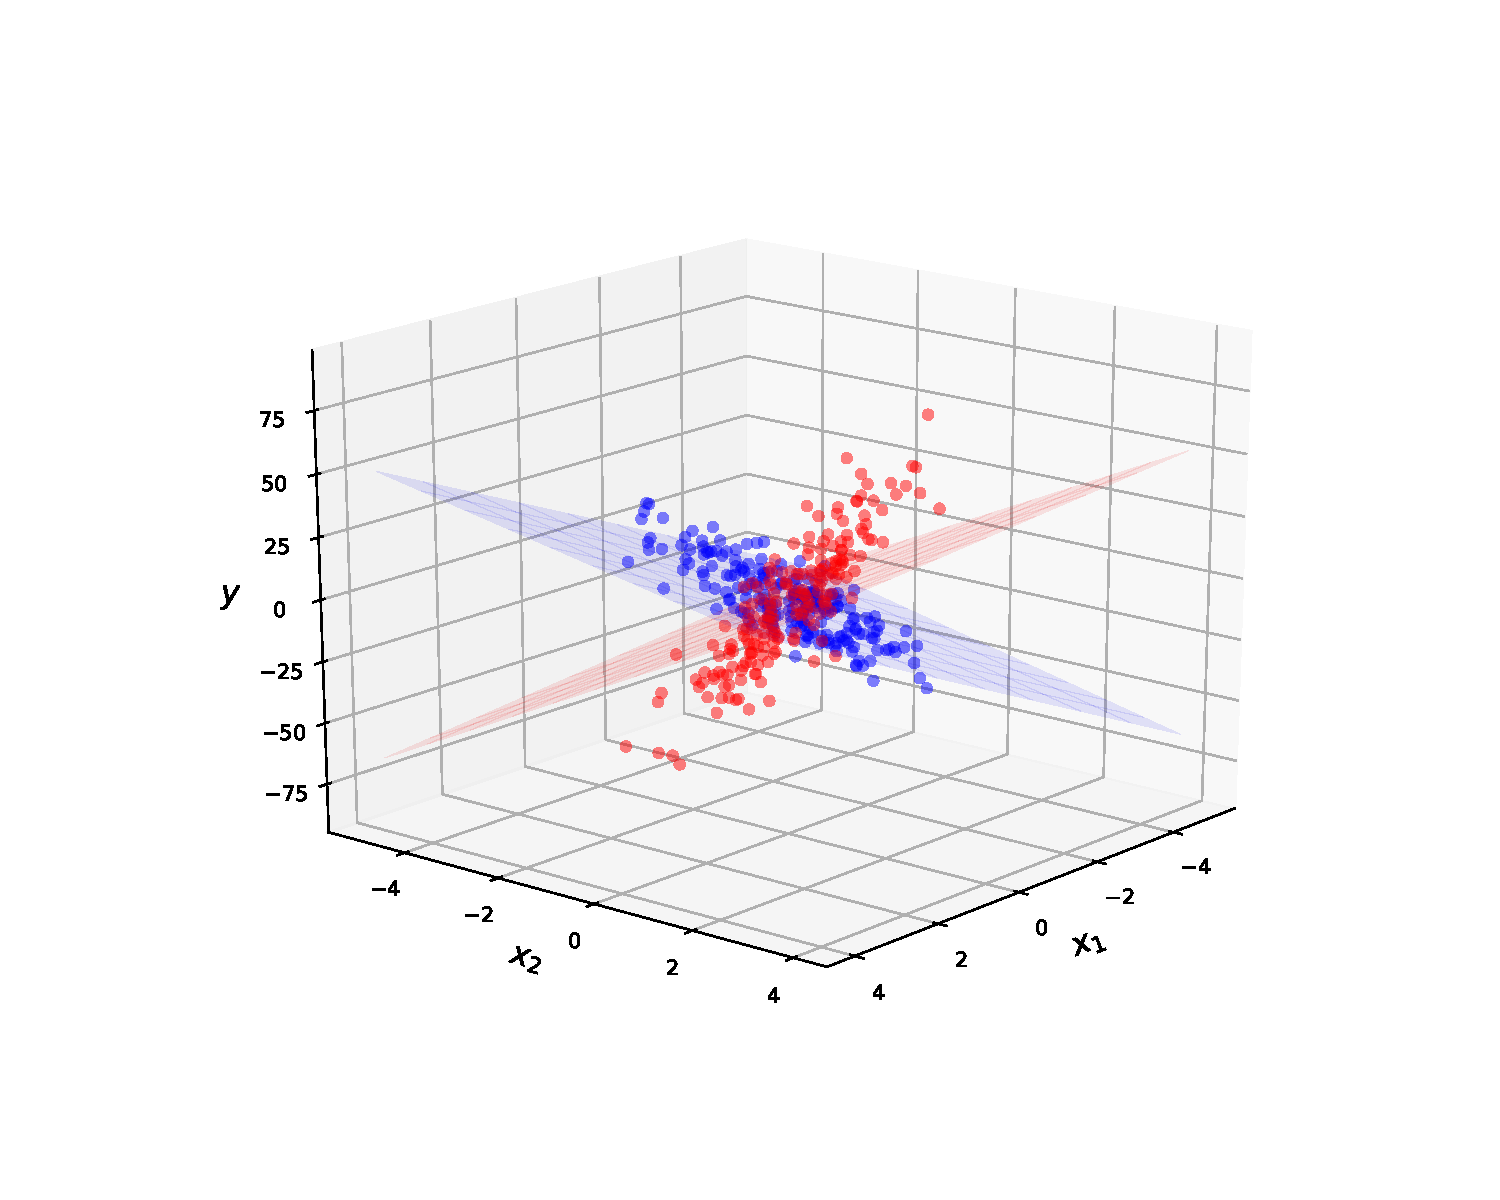
\includegraphics[width=1.2\linewidth]{experiment1-random.pdf}  б) \end{center}
\end{minipage}
\caption{а) Признаки, соответствующие другому подмножеству, заполнялись нулями, б) признаки, соответствующие другому подмножеству, заполнялись случайными числами. Точки соответствуют правильным ответам, плоскости задают предсказание линейной модели для каждого из подмножеств.}
\label{ris:image1}
\end{center}
\end{figure}


Данный эксперимент показывает, что для аппроксимации выборки, порожденной несколькими источниками, одна модель не подходит. Таким образом, при построение модели для обучения нужно учитывать гипотезу порождения данных. Нередко оказывается, что данные порождены несколькими источниками. В этом случае для лучшей аппроксимации можно использовать ансамбль локальных моделей, где каждая локальная модель обрабатывает свою область признакового пространства (в одной области объекты имеют схожие признаки, объекты из разных областей имеют разные признаковые описания).

\subsection{Базовый алгоритм. Построение ансамбля локальных моделей}

Данный эксперимент ставится для того, чтобы показать, что ансамбль локальных моделей может быть использован в случае, когда выборка порождена несколькими источниками, и лучше аппроксимирует выборку, чем одна модель.


В данном эксперименте для аппроксимации используется ансамбль двух линейных локальных моделей. 

В первом эксперименте ансамбль обучается на выборке $(\mathbf{y}, \mathbf{X}$, а во втором --- на выборке $(\mathbf{y}, \mathbf{\hat{X}}$. Ансамбль двух линейных локальных моделей хорошо аппроксимирует выборку (см. рис. $2$ а, б).  

\begin{figure}[h]
\begin{center}
\begin{minipage}[h]{0.49\linewidth}
\begin{center}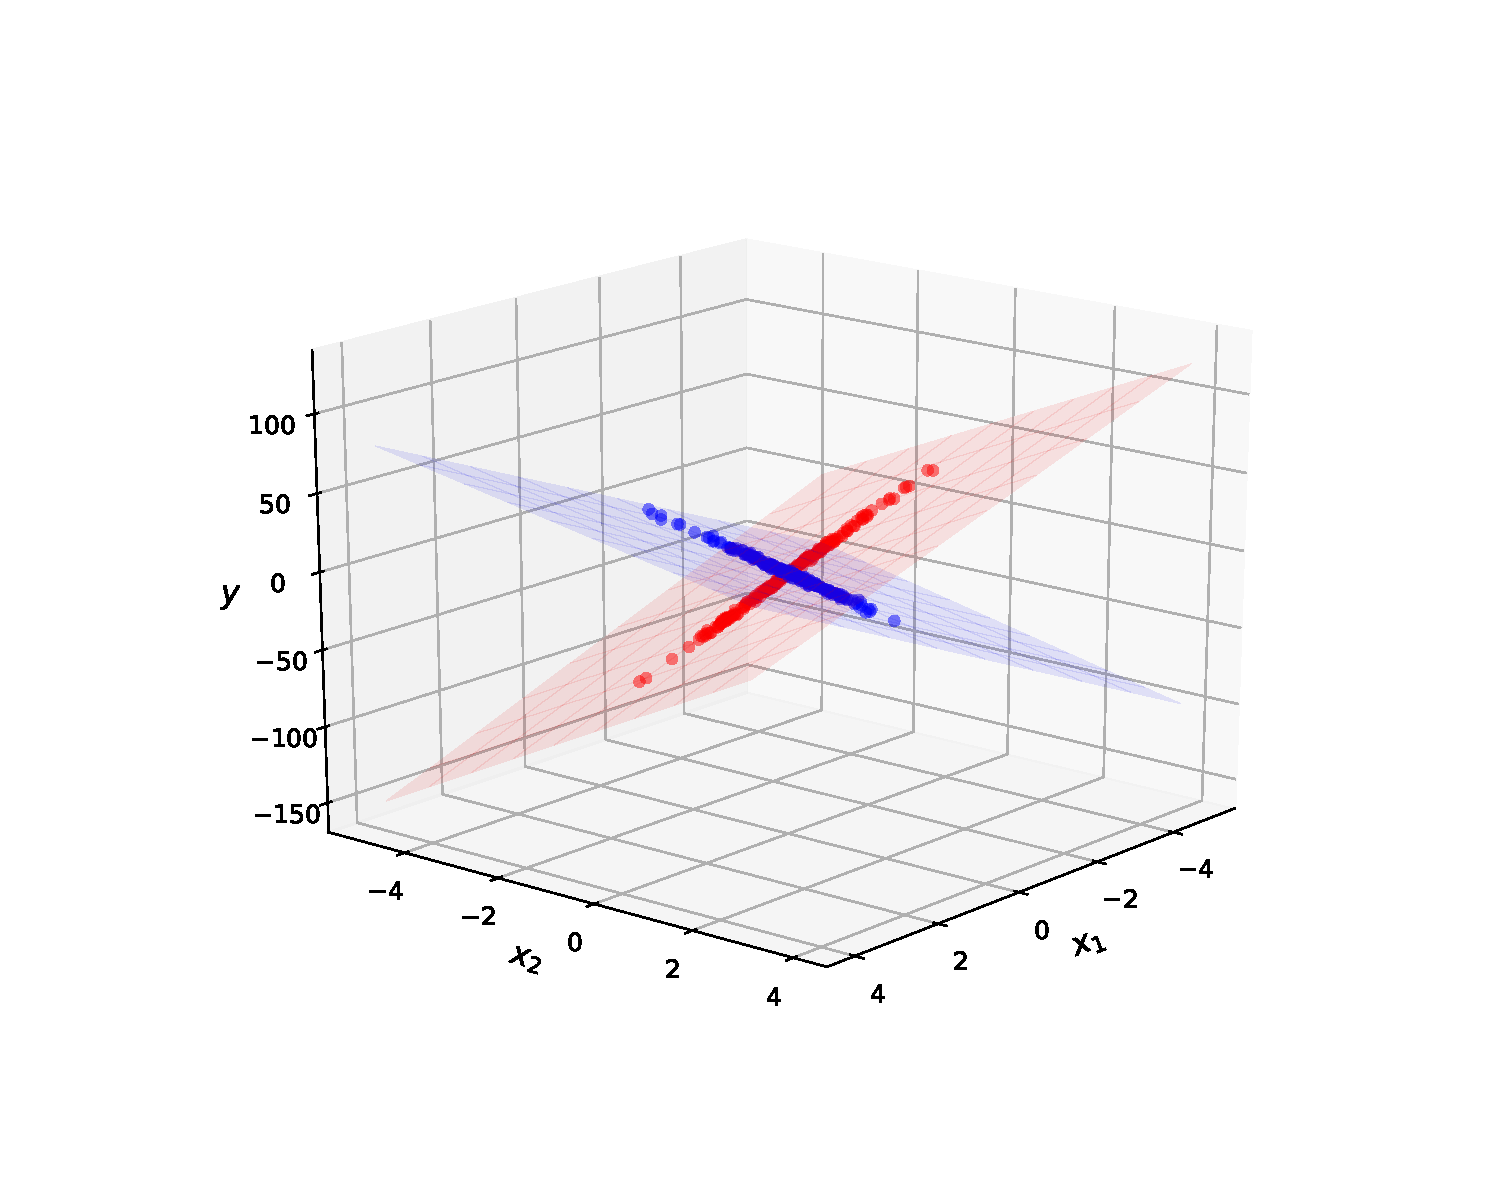
\includegraphics[width=1.2\linewidth]{experiment2-zeros.pdf}  а) \end{center}
\end{minipage}
\hfill
\begin{minipage}[h]{0.49\linewidth}
\begin{center}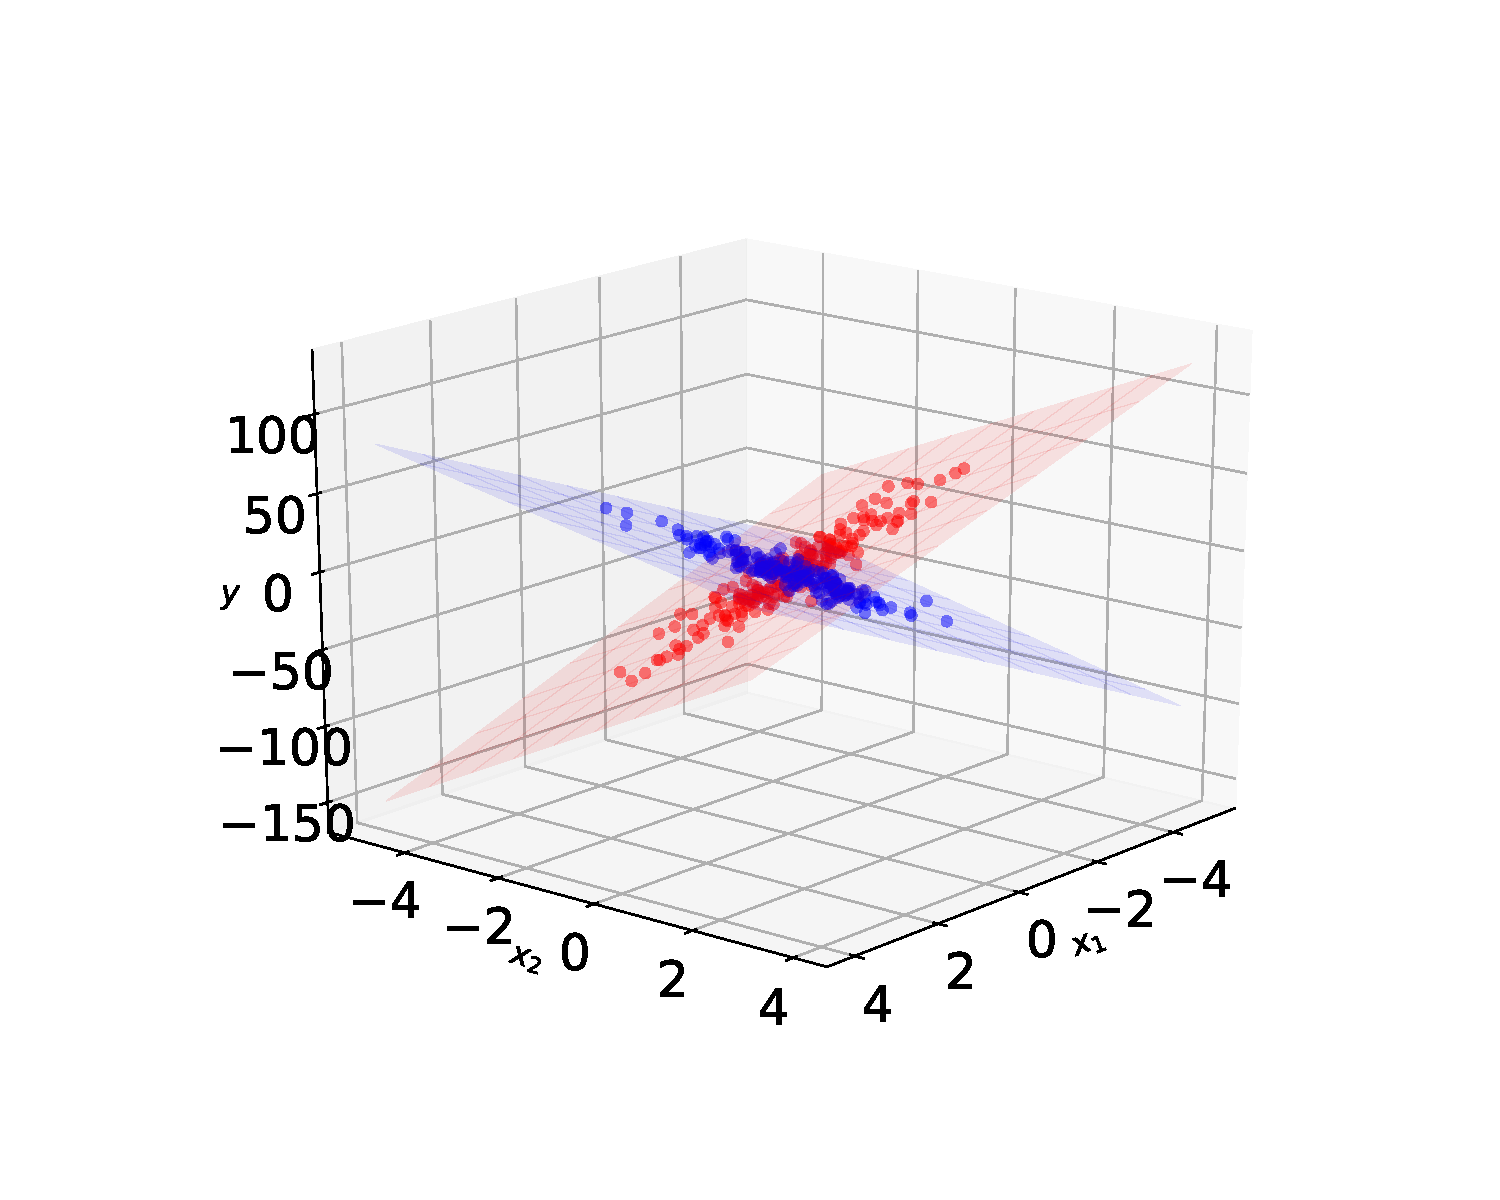
\includegraphics[width=1.2\linewidth]{experiment2-random.pdf}  б) \end{center}
\end{minipage}
\caption{а) Признаки, соответствующие другому подмножеству, заполнялись нулями, б) признаки, соответствующие другому подмножеству, заполнялись случайными числами. Точки соответствуют правильным ответам, плоскости задают предсказание мультимодели для каждого из подмножеств.}
\label{ris:image1}
\end{center}
\end{figure}

Данный эксперимент показывает, что для аппроксимации выборки, порожденной несколькими источниками, подходит ансамбль локальных моделей. Качество аппроксимации ансамбля моделей выше, чем при использовании лишь одной модели. 


\bibliographystyle{unsrt}
\bibliography{Islamov}

\end{document}
